%!TEX root = ..\Gus-thesis.tex
\glsresetall

\chapter{Introduction} \label{chap:Introduction}

%\vfill{}

% Context:Metrology One of the objectives in metrology is the estimation of the true value of physical quantities.
A measurement is a dynamic process, and a sensor is a dynamic system.
The physical quantities of interest are the inputs of the system, and the outputs are the electrical signals collected from the sensor.
The inputs interact with the sensor, and there are energy transfers between them that modify the sensor state.
The sensor output response depends on the applied inputs and on the sensor's initial conditions.

\color{blue}

Take for example the case of a thermometer.
To measure temperature, the thermometer is put in contact with the substance or object of interest.
According to the Newton's law of cooling, the temperature $y$ of the thermometer changes proportionally to its difference with the temperature $u$ of the matter under study:
\begin{equation}  \dfrac{dy}{dt} = k_{\mathrm{T}} \left( u - y \right) \label{eqn:NewtonCooling} \end{equation}
where the proportionality constant $k_{\mathrm{T}}$ is a parameter of the thermometer's first order model.
The input $u$ is unknown and its estimation is the objective of the measurement.
It is customary to take the reading from the thermometer once the temperature stops changing. 

Another popular example of a measurement is found in weighing. 
In most of modern scales, the object of interest is placed on top of a weighing sensor.
A simple model of the weighing sensor is a second order mass-spring-damper model shown in Figure \ref{fig:simple_msd_system}.
In this model, the unknown mass $u(t)$, that can be time-dependent, causes a displacement $y$ of the scale and the dynamics of the sensor are described by the differential equation:
\begin{equation} \dfrac{d}{dt} \left( \left(u(t)+m\right) \ \dfrac{dy}{dt} \right) + k_{\mathrm{d}} \dfrac{dy}{dt} + k_{\mathrm{s}} y = \left(u(t)+m\right)  g \end{equation}
where $m$ is the own mass of the scale, $k_{\mathrm{d}}$ is the damping constant, $k_{\mathrm{s}}$ is the elasticity constant, and $g = 9.81$ $\mathrm{m/s}^2$ is the gravitational acceleration. 

For illustration purposes, Figures \ref{fig:thermometer} and \ref{fig:scale} show the responses of the thermometer and the weighing sensors, respectively, after the application of a constant input $u$, which can be represented by a step input. 

\begin{figure}[htb!]
\centering

\begin{tikzpicture}[every node/.style={draw,outer sep=0pt,thick}]
\tikzstyle{spring}=[thick,decorate,decoration={zigzag,pre length=0.3cm,post length=0.3cm,segment length=6}]
\tikzstyle{damper}=[thick,decoration={markings,  
  mark connection node=dmp,
  mark=at position 0.5 with 
  {
    \node (dmp) [thick,inner sep=0pt,transform shape,rotate=-90,minimum width=15pt,minimum height=3pt,draw=none] {};
    \draw [thick] ($(dmp.north east)+(2pt,0)$) -- (dmp.south east) -- (dmp.south west) -- ($(dmp.north west)+(2pt,0)$);
    \draw [thick] ($(dmp.north)+(0,-5pt)$) -- ($(dmp.north)+(0,5pt)$);
  }
}, decorate]
\tikzstyle{ground}=[fill,pattern=north east lines,draw=none,minimum width=0.63cm,minimum height=0.3cm]

\node (M) [minimum width=2.5cm,minimum height=0.05cm] {$m$};
\node (Mu) [minimum width=2.5cm,minimum height=0.75cm,yshift=0.57cm] {$u(t)$};

\node (ground1) at (M.south) [ground,yshift=-1.5cm,xshift=-0.625cm,anchor=north] {};
\draw (ground1.north west) -- (ground1.north east);
\draw [spring] (ground1.north) -- ($(M.south east)!(ground1.north)!(M.south west)$);

\node (groundc) at (M.south) [ground,yshift=-1.5cm,anchor=north] {}; 
\draw (groundc.north west) -- (groundc.north east);

\node (ground2) at (M.south) [ground,yshift=-1.5cm,xshift=0.625cm,anchor=north] {};
\draw (ground2.north west) -- (ground2.north east);
\draw [damper] (ground2.north) -- ($(M.south east)!(ground2.north)!(M.south west)$);

\node[draw=none,fill=none] at (-0.9cm,-1cm) {$k_{\mathrm{s}}$};
\node[draw=none,fill=none] at (0.15cm,-1cm) {$k_{\mathrm{d}}$};
\node[draw=none,fill=none] at (2.0cm,1.0cm) {$y$};
\draw [-latex,thick]  ++(2.2cm,-1cm) -- +(0cm,2.25cm);

\draw [-latex,thick] (M.east) ++(0,0) -- +(1cm,0);
\draw [line width=0.25mm] (2.2cm,-1cm) -- (2.2cm,1cm);
\draw [line width=0.25mm] (2.1cm,-1cm) -- (2.3cm,-1cm);
\draw [line width=0.25mm] (2.1cm,1cm) -- (2.3cm,1cm);
\draw [line width=0.25mm] (2.1cm,-0.5cm) -- (2.3cm,-0.5cm);
\draw [line width=0.25mm] (2.1cm,0.5cm) -- (2.3cm,0.5cm);
\draw [line width=0.25mm] (2.15cm,-0.25cm) -- (2.25cm,-0.25cm);
\draw [line width=0.25mm] (2.15cm,0.25cm) -- (2.25cm,0.25cm);
\draw [line width=0.25mm] (2.15cm,-0.75cm) -- (2.25cm,-0.75cm);
\draw [line width=0.25mm] (2.15cm,0.75cm) -- (2.25cm,0.75cm);
\draw [line width=0.25mm] (2.1cm,0cm) -- (2.3cm,0cm);

\end{tikzpicture}

\caption{\label{fig:simple_msd_system} \color{blue} A second order mass-spring-damper model represents the weighing sensor. The application of the mass $u$ causes a change in the position $y$ of the scale. \color{black} } 
\end{figure}


\begin{figure}[!htbp]
\centering
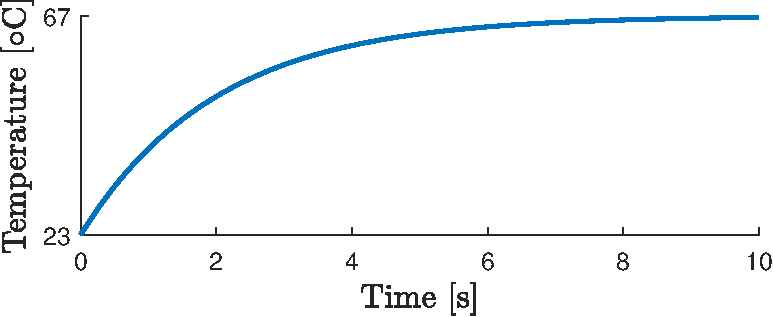
\includegraphics[width=0.69\columnwidth]{./ChapterIntroduction/fig/Fig_2.pdf} 
\caption{ \label{fig:thermometer} 
\color{blue} This simulation shows an example of the temperature change experimented by a thermometer, with $k_{\mathrm{T}}=0.5 s^{-1}$, caused by a step input of 67 $^{\circ} \mathrm{C}$  when the thermometer was initially at 23 $^{\circ} \mathrm{C}$. In this example, we should wait 10 s to have an estimation of the input with a relative error lower than 0.5\%. \color{black} }
\end{figure}

\begin{figure}[!htbp]
\centering
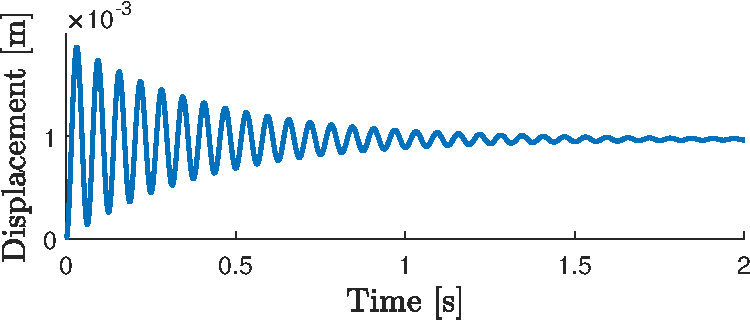
\includegraphics[width=0.69\columnwidth]{./ChapterIntroduction/fig/Fig_3.pdf} 
\caption{ \label{fig:scale} 
\color{blue} This simulation illustrates the displacement observed when a constant input $u=1 \mathrm{kg}$ is applied to a weighing sensor in equilibrium. The sensor parameters are $k_{\mathrm{d}} = 5 \ \mathrm{N \ s/m}$, $m = 5 \ \mathrm{g}$, and $k_{\mathrm{s}} = 10250 \ \mathrm{N/m}$. In this conditions, the user has to wait more that 2 s to observe a stabilization on the scale and to estimate the mass from reading the final value of the displacement with a relative error smaller than 0.72\%. \color{black}  }
\end{figure}

In \citet{Eichstadt12} an illustration on a force measurement sensor can be found. 
The sensor is modeled as a cascade of two damped mass-spring systems. 
The transfer function of the sensor is $H(s) = H_1(s) \ H_2(s)$, where each of the two transfer functions are described by
\begin{equation} H_i(s) = \dfrac{\left( 2 \pi f_{0,i}\right)^2}{s^2  + 2 \delta_i \left( 2 \pi f_{0,i}\right) s  +  \left( 2 \pi f_{0,i}\right)^2} 
\end{equation}  
where $\delta_1 = 0.1$, $\delta_2 = 0.2$, $f_{0,1} = 1.9$ Hz, and $f_{0,2} = 7$ Hz are the system parameters.
The response of this sensor to a unit step input, shown in Figure \ref{fig:force}, takes at least 5 s to in which the transient response is predominant.  

\begin{figure}[!htbp]
\centering
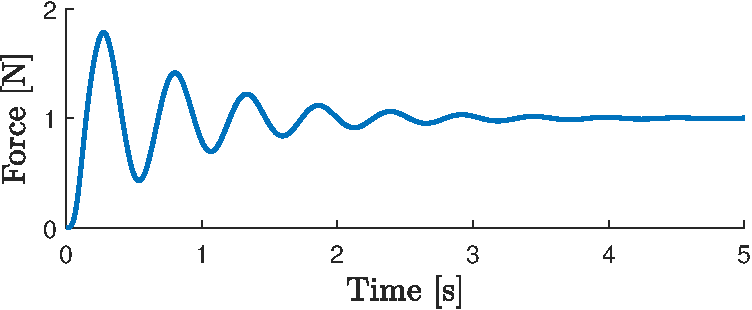
\includegraphics[width=0.69\columnwidth]{./ChapterIntroduction/fig/Fig_4.pdf} 
\caption{ \label{fig:force} 
\color{blue} The simulation of a force sensor based on a double mass-spring system in cascade also shows that the stabilization after a unit step input is not instantaneous. In the plot we infer that the user has to wait 5 s to estimate the force from the sensor response that is 0.25\% far from its value in equilibrium. \color{black}  }
\end{figure}

The handbook of sensors written by \citet{Fraden16Book} describes a pressure sensor that detects sudden changes in the pressure inside a room.
These changes can be caused by the opening of a door or by the movement of a person.
The principle of operation of detecting minute pressure gradients is the flowmeter that compares the pressure at both outlets of a tube.   
An experimental identification of such a flowmeter is described in \citet{Wiklund02}, where a second order model is proposed to explain the dynamics with the transfer function
\begin{equation} H(s) = \dfrac{ e^{-\tau_{delay}s}}{\left( 1 +  \tau_1 s \right) \left( 1 +  \tau_2 s \right)} 
\end{equation}  
where $\tau_{delay} = 0.07$ s is the dead time, and $\tau_{1} = 0.01$ s and $\tau_{2} = 1.6$ s are two time constants.
The step response simulation of this dynamic model results in the sensor step response shown in Figure \ref{fig:pressure}.  
We have a response to a unit step function that is mostly and increasing exponential that requires 7 s approximately to reach a value that is 98.7\% of its maximum value.

\begin{figure}[!htbp]
\centering
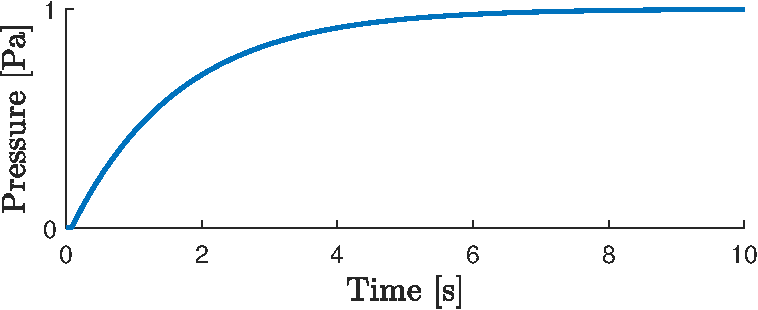
\includegraphics[width=0.69\columnwidth]{./ChapterIntroduction/fig/Fig_5.pdf} 
\caption{ \label{fig:pressure} 
\color{blue} The response of a flowmeter to a sudden change in its pressure gradient acrros the extremes of a tube is an overdamped transient response. Ideally we would expect the the transient response follows closely the shape of the unit step input applied, but instead an exponential response is observed, that last for more than 7 s.  \color{black}  }
\end{figure}

\color{black}


% Context:Tradeoff speed vs accuracy
There is a trade-off between speed and accuracy when measuring with a linear time-invariant sensor.
The input excitation drives the sensor into a transient regime, and when the transient response is below the noise level, we say that the sensor is in steady state.
During the sensor transient regime, the response does not directly represent the input, but 
in steady state, the sensor response is proportional to the excitation.
The input can be estimated accurately from the sensor steady state response using the sensor static gain.
However, waiting for the steady state is not always possible for practical applications that need fast measurements.
In these practical applications, the input must be estimated during the transient regime.

% Context:Compensation systems, 
One approach to get a fast input estimation is filtering the sensor transient response with another dynamical system that inverts the dynamics of the sensor.
The filter output is an input estimate that compensates for the time span of the sensor transient regime.
The transient duration of the compensation filter should be smaller than that of the sensor.
The compensator is designed after a sensor model to deconvolve the sensor response.

% Context:Digital signal processing
Another approach relies on the use of digital signal processors (DSP) to estimate the input value from the sensor transient response.
DSPs offer an extra versatility level since they allow to implement methods that do not necessarily simulate the dynamics of linear systems, such as digital filters.
A suitable data-driven method in a DSP can provide faster input estimations than with the model-based compensators.

% Context:Data-driven step input estimation method
An example of a data-driven method devised for a DSP is the direct step input level estimation from the sensor step response introduced in \citet{Markovsky15cep}.
This method formulates a Hankel structured errors-in-variables (EIV) problem with correlation.
The regression matrix has a block-Hankel structure.
The correlation exists because the transient response, perturbed by measurement noise, constructs both the regression matrix and the regressor.
The measurement noise is assumed to have zero mean and finite variance.
The method is implemented in real-time using a recursive least-squares (RLS) solution of the structured EIV problem.
% Avoiding the model identification from input-output data and directly estimating the input from the transient response reduces the input estimation time and makes data-driven input estimation methods suitable for real-time 

% Context:Data-driven methodology
% The philosophy behind the estimation method is avoiding the explicit identification of a system model from input-output data and estimating directly the input from the transient response.
The main advantage of the data-driven step input estimation method is that it does not identify the sensor model, but instead, it directly estimates the input. 
The direct estimation differs from the standard two-stage methodology that first identifies the sensor model and later estimates the input.
In this approach, the output-error (OE) problem is converted into an EIV problem that is harder to solve, but the RLS solution is easy to compute.
The range of application of the data-driven input estimation method is extensive because it is independent of the sensor model.
The main disadvantage of the data-driven input estimation method is that its stochastic properties are not straightforwardly evident. 
It is more complex to find the stochastic properties of EIV problems when they have structure and correlation.
% Moreover, the online uncertainty assessment may not be feasible and we have to rely on confidence bounds.


% Problem under study: Dynamic measurements
% DM:Uncertainty assessment of data-driven input estimation methods
% DM:Experimental validation of the data-driven step input estimation method
The estimation uncertainty assessment is needed to validate the estimation methods for metrology applications.
The uncertainty of the data-driven step input estimation method described in \citet{Markovsky15ieee} is unknown.
The estimation bias and variance define the estimation uncertainty, as it is explained in \citet{Pintelon12Book}, and they can be obtained by conducting an elementwise statistical analysis. 
The validation of the step input estimation method requires also to demonstrate its effectiveness on real-life measurements.
Temperature and mass sensors are suitable for real-life measurement experiments.
One challenge of using real-life sensor outputs is that the noise may not fulfill the whiteness assumed in the estimation problem formulation and in the statistical analysis.
The experimental and simulation results permit to evaluate the step input estimation method performance.

% DM:Estimation of affine input parameters
The step input estimation method concepts raise the curiosity towards the design of estimation methods for other input models.
The affine input model, for example, is found in conveyor dynamic weighing systems.
The dynamic weighing estimates the mass of materials or products during their transportation.
When the conveyor belt moves at a constant speed, the weighing sensor is excited with an affine profile, 
described by the slope and the intercept parameters.
The affine input parameters can be estimated by adapting the step input estimation method.

% general preview of the thesis contents
%This thesis describes three works initiated after the data-driven step input estimation method.
%The first work is a statistical analysis to elucidate the bias and the covariance of the estimate that this method provides.
%These statistical moments build the estimation uncertainty that appraises the effectiveness of the method.
   
 
\section{State of the art}

The scientific literature contains metrology studies that deal with the dynamic process effects of measurements.
This subsection presents a list of relevant works published in relation with the thesis topic. 
These works study theoretical aspects like the estimation of inherent dynamical errors presented in \citet{Hessling06}, the dynamic correction in time domain proposed in \citet{Hessling08a}; and experimental aspects like the increment of the amount of sensors in production lines for quick decision making in autonomous control described in \citet{Esward09}.  

To implement input estimation methods in the practice, the compensation filters based on deconvolution explained by \citet{Eichstadt10} are the preferred methodology to develop, for example, 
analog filters in \citet{Jafaripanah05}, 
adaptive digital filters in \citet{Shu93}, 
lattice adaptive filters in \citet{Hernandez06}, 
compensators for simultaneous responses of different sensors in \citet{Boschetti13}, 
regularized deconvolution compensators in \citet{Dienstfrey14}, 
and a multiple choice set of filters in \citet{Huang16}. 
All these methods have in common the use of the measurement system model parameters to build the compensator.


% Digital signal processing estimation methods
A list of measurement methods based on digital signal processors (DSP) include 
a data-driven dynamic error correction and its impact on the measured temperature studied in \citet{Saggin01},
a modulation quality measurement of microwave access systems presented in \citet{Angrisani10}, 
a real-time rotational speed estimation method using correlation introduced in \citet{Wang14},
a biology-inspired electronic nose developed in \citet{Jing16},
and impedance measurements for material damage estimation method using cross-correlation introduced in \citet{deCastro19}.
The data-driven step input estimation method proposed by \citet{Markovsky15cep} is added to this list, highlighting the fact that it can be implemented for the measurement of different physical magnitudes because it is model-independent.


% Uncertainty assessment 
In metrology, a measurement is an estimation, represented as a random variable.
The measurement noise always exists, and therefore, the input estimation is commonly expressed with its two first statistical moments as it is described in \citet{Ferrero06}.
The guidelines listed in \citet{GUM08}, and accepted by the metrology community, recommend the standardization of the uncertainty assessment.
The typical measurement uncertainty analysis \color{blue} is \color{black} reviewed in \citet{daSilva12}.
The Monte Carlo method is an uncertainty evaluation tool according to \citet{Cox06},
that supports the use of simulation techniques for quantifying measurement uncertainties as suggested by \citet{Esward16}.
One example of the Monte Carlo method application is a dynamic measurement uncertainty evaluation of clinical thermometers described in \citet{Ogorevc16}.

Nevertheless, researchers like \citet{Esward09}, and \citet{Hessling10} still pinpoint the need to study more the uncertainty assessment methods.
\citet{Diniz17} recommends to consider the uncertainties of all the measurement chain components, and to avoid the direct uncertainty propagation from the calibration towards the to-be-measured quantity.  
Methods for evaluating the uncertainty associated with the output of compensation filters have been investigated for
a discrete-time infinite-response filter in \citet{Link09},
a discrete-time finite-response filter in \citet{Elster07, Elster08}, and
the Kalman filter in \citet{Eichstadt16b}.
All these works propagate the uncertainty through the filter, but it is also necessary to upward the propagation up to the sensor model to include all systematic error contributions, as it is explained by \citet{Hessling11}.



\section{Original contributions \color{blue}and organization of the thesis\color{black}}

% Preview of the thesis contents and location of the developed topics in relation to the state of the art 

This thesis describes research work initiated after the data-driven step input estimation method proposed by \citet{Markovsky15cep}.
This method aims for metrology applications but it lacked an uncertainty assessment, and, therefore, its appropriateness was questionable.
\color{blue}A description of the data-driven step input estimation method is presented in Chapter 3\color{black}.

\subsection{Statistical analysis}

\color{blue}Chapter 4 describes \color{black} the first research work conducted that is a statistical analysis of the data-driven step input estimation method, aiming to elucidate the bias and the covariance of the input estimation.
After obtaining these statistical moments, the estimation uncertainty was assessed, and thus, the effectiveness of the method was appraised.

The data-driven step input estimation method formulates a structured errors-in-variables (EIV) problem.
In linear estimation EIV problems, the measurement noise perturbs the regression matrix and the regressor, as it is detailed in \citet{VanHuffel91Book} and \citet{Markovsky07overview}.
The regression matrix, in structured EIV problems, has a structure that depends on the problem formulation.
Hankel and Toeplitz matrices appear in several application problems such as those described by \citet{Markovsky15cep} in metrology, by \citet{Soderstrom07} in system identification, by \citet{Feiz17} in image restoration, by \citet{Cai16} in nuclear magnetic resonance spectroscopy, by \citet{Pan18} in direction-of-arrival estimation, and by \citet{Jia18} in time-of-arrival estimation.

The data-driven step input estimation method introduced by \citet{Markovsky15cep} directly estimates the input from the sensor transient response. 
The perturbations in the formulated EIV problem come from the sensor output, since it is the only observed signal, and from this signal both the regression matrix and the regressor are built.
The structure in the regression matrix is block-Hankel.
The data-driven direct estimation methodology  estimates the input faster than the classical two-stage approach described in \citet{Azam15} and \citet{Niedzwiecki16a}, which first identifies a sensor model and later estimates the input using the sensor model.

Instead of using a total least-squares (TLS), \color{blue} or an intrumental variables \color{black}, solution of the structured EIV problem, the step input estimation method uses the recursive least-squares solution (RLS). 
In the review conducted by \citet{Markovsky07overview} it is shown that the TLS solution of unstructured EIV problems is consistent when the perturbations have zero mean with a given positive definite covariance, and
the TLS solution is equivalent to the maximum likelihood (ML) solution when the disturbances of the EIV problems are i.i.d. normally distributed. 
\color{blue} The classical TLS solution is obtained using singular value decomposition of the augmented matrix built from the regression matrix and the regressor as additional columns\color{black}.
However, the studies presented in \citet{VanHuffel07TLSeditorial} demonstrate that the structured TLS solutions cannot be generalized since each structure in an EIV problem requires a specific treatment. 
Moreover, the ML estimator of structured EIV problems leads to non-convex optimization, and the global optimum is not guaranteed \cite{Beck10}.
\color{blue} On the other hand, the instrumental variable (IV) solution of EIV problems use an additional variable.
The additional variable is an instrument with the purpose of removing the bias of the estimate.
To do this, the construction of the instrumental variable has to be done in such a way that it is uncorrelated with the perturbations and correlated with the regressor, as it is described in \citet{Soderstrom18}. 
\color{black} 
Unfortunately, the computational complexity of the TLS, ML, and IV solutions inhibits their real-time implementation.

\color{blue} 
The solution of the step input estimation problem is preferred to be online, since its applications are in the field of metrology.
In the literature there are references for online implementations of TLS, ML or IV methods, which are are mainly recursive versions of the solution methods.
These recursive versions are developed to solve EIV problems for system identification and fault detection.
We have, for example, the generalized recursive TLS solutions introduced in \citet{Rhode14recursive} and \citet{Rhode14recursivecov}, and the recursive IV solutions developed in \citet{Djouambi12}, \citet{Shang16} and \citet{Gil15}.
These methods cannot be used as off-the-shelf solutions to the step input estimation EIV problem because they need to be adapted to the specific requirements of the problem.
One is that the sensor output is the only measured signal, since the input is to-be estimated, and the solution should be simpler, preferable with a linear complexity $O(n)$, instead of the cubic $O(n^3)$ or cuadratic $O(n^2)$ complexities of the mentioned recursive methods, where $n$ is the sensor order.
The proposal of the data-driven step input estimation method includes the recursive least-squares (RLS) solution.
Compared with recursive TLS or recursive IV solutions, RLS is a suboptimal but more simple solution to the structured EIV problem with lower computational complexity,  suitable for real-time implementation.
\color{black} 


The previously published works that propose LS estimators to solve structured EIV problems do not study the required statistical moments to know the uncertainty of the data-driven step input estimation method.
In the literature we find 
the design of a fast algorithm for matrices with small displacement rank in \citet{Mastronardi07fast}, 
the study of the LS estimator consistency in \citet{Palanthandalam10parameter},
the determination of the bias, and the mean squared error of the parameter estimates in the identification of AR models in \citet{Kiviet12high}, \citet{Kiviet14improved}, and
a discussion of the causes of bias and inconsistency in homogeneous estimators in \citet{Yeredor04homogeneous}.
The literature does not address the uncertainty of LS estimators for structured EIV problems.

The uncertainty of an estimation method is expressed in \citet{Pintelon12Book} using the bias and covariance of the estimate.
To know the uncertainty of the data-driven step input estimation method, we quantified the bias and covariance of the LS solution of EIV problems, for unstructured and structured cases. 
The bias and covariance quantification extend the perturbation analysis that was investigated in \citet{Stewart90SPT} and in \citet{Vaccaro94}.
The conducted analysis provides insight into the impact that the structure and the correlation have on the LS estimation uncertainty.
The study presented in this thesis illustrates a methodology to conduct statistical analysis for any structured EIV problem.

We derived expressions that quantify the bias and covariance by obtaining the mathematical expectation of the LS estimate approximated by the second-order Taylor series expansion.
Using Monte Carlo simulations, we validated the accuracy of the bias and covariance expressions.
These expressions estimate the bias and covariance that the data-driven step input estimation method will exhibit for a given sample size and perturbation level.
We compared in \citet{QuintanaCSDA} the mean squared error of the LS estimate to the minimum variance specified by the Cram\'er-Rao lower bound of the structured EIV problem, to determine the conditions under which the data-driven step input estimation method is appropriate for practical applications.

\subsection{Experimental validation}

\color{blue}Chapter 5 describes \color{black} the second research work that consisted in a series of experiments conducted to validate the data-driven step input estimation method in real-life applications.
The experiments were realizations of the step input excitation using a mass sensor.
The step input estimation method showed robustness when the measurement noise is not Gaussian and white, as it was assumed in the theoretical analyses.

The validation of the data-driven step input estimation method in a practical application was necessary to demonstrate the usefulness of the method.
The method performance was studied in \citet{Markovsky15cep} using simulations and temperature experiments on a digital signal processor (DSP) of low cost.
The method estimates the unknown level of step inputs by processing the sensor step response, and 
avoiding the sensor modeling stage.
The formulation of the estimation method is a correlated errors-in-variables (EIV) problem with block-Hankel structure.

Other methods for input estimation mainly compensate the sensor transient response, for example, by 
recursive estimation of the compensator parameters in \citet{Shu93}, 
finite impulse response (FIR) filtering in \citet{Elster07}, \citet{Niedzwiecki16b} and 
infinite impulse response (IIR) filtering in \citet{Pintelon90}, \citet{Elster08}.
The uncertainty propagation for these model-based compensators is based on the transfer function or state-space representations of the LTI sensor and filter systems in \citet{Link09} and \citet{Hale09}.
Another way to assess the measurement uncertainty is by observing the results of multiple practical measurements as it is described in \citet{Pietrzak14} for mass and in \citet{Ogorevc16} for temperature sensors.

To validate the data-driven step input estimation method we built a weighing system setup based on a load cell sensor.
The weighing setup was constructed to ensure repeatability and reproducibility, along with different experimental realizations.
Load cell sensors are versatile devices that are applied for
heart and breathing physiological signal monitoring in \citet{Lee16},
clinical analysis of sleep quality in \citet{Zahradka18},
automobile safety studies in \citet{Ballo16},
wind turbine design in \citet{Rossander15}, 
civil engineering structure studies in \citet{Olmi16}, and 
sport bicycle design in \citet{Casas16}, to name a few.


\begin{comment}
% Load cell sensors 
Weighing has been basic for the development of scientific and trade activites. 
The load cell is now a standard transducer for weight determination and also for the improvement of measurement techniques, such as the geometric approach to processing of load cell responses \citet{Kesilmis16}, the design of new conveyor machinery \citet{Yamani18}, and electronic truck scales \citet{Guo18}.

In safety studies, a six axis load cell is devised to quantify accelerations and impact forces exerted on a dummy \citet{Ballo16}.
In alternative energy developments the load cells are useful to measure the forces on the arms of a vertical axis wind turbine \citet{Rossander15}.
An academic study of the load that a structure withstands is conducted with strain gage load cells that confirms the numerical results and facilitates the design of complex shaped structures \citet{Olmi16}.
In sports, the performance of new instrumented crank mechanisms is fostered by the utilization of load cells in the characterization, analysis and validation design stages \citet{Casas16}.

The versatility of the load cells permits the physiological signal monitoring of the the heart and breathing rates \citet{Lee16}, clinical analysis of sleep quality \citet{Zahradka18} and the classification of the movement intensity of people while they are sleeping \citet{Alaziz17}. 
All of these experimental studies have load cells installed on bed setups.


%
An extension of the methodology proposed for the data-driven step input estimation was formulated to estimate the parameters of an affine input that changes at a constant rate,  by signal processing of the sensor transient response.
This type of ramp inputs is observed in the measurement of mass during the transportation of products on conveyor systems, ranging from few grams \citet{Burmen09} to almost hundreds of kilograms \citet{Tasaki07}.
The data-driven affine input estimation method is proposed as an alternative to existing compensation filters, such as 
the time-variant low-pass filters introduced in \citet{Piskorowski08, Pietrzak14}, and
the combination of filters in cascade proposed in \citet{Niedzwiecki16a}.
\end{comment}


The signal from the load cell sensor in the weighing system is conditioned using operational amplifiers.
The signal conditioning amplifier has a low-pass filter to prevent aliasing from the noise.
The observed measurement noise has non-white noise properties, mainly due to the characteristics of the load cell sensor.
One of the assumptions of the step input estimation method formulation is that the measurement noise is Gaussian and white. 
Nevertheless, the estimation results discussed in \citet{QuintanaTIM} show that the method is still able to provide useful input estimations.

The empirical bias and covariance obtained after repeating the weighing experiment was compared to the bias and covariance estimations obtained in our previous research work (\citet{QuintanaCSDA}), and to the minimal variance given by the  Cram\'er-Rao lower bound (CRLB) of the structured EIV problem.
We found that the mean squared error (MSE) of the step input estimate is near the CRLB, and the distance between the MSE and the CRLB provides a confidence interval for the input estimate with respect to the level of the measurement noise. 

 
\subsection{Affine input estimation}

\color{blue}Chapter 6 describes \color{black} the third research work conducted to estimate the parameters of an affine input, following the data-driven approach for real-time applications. 
The data-driven method uses exponential weighing in the recursive least-squares solution of a structured errors-in-variables problem, to give preference to recent samples over the older samples.
The methodology and performance of the data-driven affine input estimation method were compared to those of a maximum-likelihood method.

A dynamic measurement is present when the fluctuations of the measurand impact on the input estimation, such as when a low-bandwidth sensor is excited with a fast changing input.
The detection of input characteristics is of interest in several scientific and industrial applications, such as those described for measuring temperature in \citet{Saggin01}, pressure in \citet{Matthews14}, acceleration in \citet{Link07}, force in \citet{Vlajic16}, \citet{Hessling08a}, and mass in \citet{Shu93}, \citet{Boschetti13}.

We developed a method to estimate the parameters of inputs that vary at a constant rate, influenced by the data-driven signal processing method that estimates the step level value using subspace techniques introduced in \citet{Markovsky15cep}, \citet{Markovsky15ieee}.
An input varies at a constant rate in applications where the magnitude of interest activates the sensor gradually. 
An example of this affine activation is the measurement of mass while the to-be-weighted object is transported by a conveyor belt, and the profile of the input is a saturated ramp.
Current solutions described in \citet{Tasaki07}, \citet{Pietrzak14} use low pass filters to estimate the mass in motion based on the saturated part of the ramp input.
The signal processing affine input estimation methods are motivated by the need to obtain the mass of the object from the ramp before it reaches saturation.

We propose in \citet{QuintanaMEAS} a data-driven method that estimates the affine input,
which is parameterized as a straight line model where the slope and the intercept are the parameters of interest.
The data-driven affine input estimation method formulates a structured errors-invariables (EIV) problem, similar to the one formulated for the step input estimation.
An exponential weight is added to the recursive least-squares.
This is a forgetting factor that considers that the newer samples are more relevant for the input parameters estimation.
The data-driven affine input estimation method is a recursive algorithm that can be implemented in real-time since it has low computational cost.

The performance of the proposed method is compared to that of a maximum-likelihood (ML) estimation method based on local-optimization and a time-varying compensation filter.
The ML method simulates the response of a sensor model to an affine input, and minimizes a cost function that is the sum of the squared differences between the actual and the simulated sensor responses. 
The ML method resembles the model predictive control approach, explained in \citet{Mayne14}, in the sense that a cost function is minimized iteratively to optimize the parameters of a sensor model using the observed sensor response in a receding time horizon.
The difference is that the ML method aims to estimate the unknown value of the affine input parameters instead of identifying a model and controlling the dynamic system. 
 
After observing the simulation results, the data-driven affine input estimation method is suitable for real-time applications since it requires low computational resources. 
The ML method is more appropriate for off-line processing of the sensor transient response, but
it can estimate also the parameters of a sensor model, and the initial conditions of the sensor.
The main drawback of the ML method is the need of high computational resources.

\subsection{\color{blue}Main findings\color{black}}
\color{blue}Chapter 7 concludes this thesis work and summarizes the main results obtained in the conducted research. 

The data-driven step input estimation method reduces the input estimation time compared with formulations based on models of the sensor.
This is because the estimation method does not require to invert the sensor dynamics.
Instead, an algorithm in a digital signal processor finds directly the step input value from the sensor response.  
Since the method is not rescricted to a particular sensor model, the method can process the step response of any sensor, and provides the input estimation in different applications. 
Moreover, the method requires relatively low computational power to process the signal of the sensor.
For these reasons, the data-driven method is suitable for real-time measurements.

After studying the statistical properties of the step input estimation, we know the accuracy (bias) and the precision (variance) of the results.
This knowlewdge allows one to understand what is the uncertainty on the step input value that the method estimates.
We have derived formulas to quantify the bias and the variance of the step input estimation.
With these formulas we can foresee the bias and standard deviation we will obtain with the method given the number of samples processed and the level of the measurement noise.

The implementation of the bias and variance calculation is illustrated with a real life sensor.
A weighing system, that uses a load cell sensor, is used to generate real life sensor step responses. 
The measurement noise observed from this weighing sensor is not Gaussian white noise.
The study of the estimation method performance with real data suggests what is the method order required to set a proper implementation. 

It was explored the applicability of data-driven methods to estimate an affine input from the sensor response.
This input model is observed in measurements where the input changes with a constant rate. 
The signal processing algorithm, studied in the previous stages of the research, was extended to solve the affine input estimation problem.   
The performance results of the extended method is compared with a maximum-likelihood method that solves the affine input estimation problem using optimization.

We learnt that the data-driven input estimation methods are simple-to-use methods that run on digital signal processors with few computational resources and estimate the unknown inputs in real time, where the estimation uncertainty can be deduced from the amount of data processed and measurement noise variance.  






\color{black}



%\newpage